\documentclass{standalone}
\usepackage[T1]{fontenc}
\usepackage{lmodern}
\usepackage{tikz}
\usetikzlibrary{arrows.meta,calc,fit,backgrounds}
\usepackage{xcolor}
\definecolor{ink}{HTML}{000000}
\definecolor{muted}{HTML}{000000}
\definecolor{teal}{HTML}{0EAAA7}
\definecolor{violet}{HTML}{6E49D2}
\definecolor{orange}{HTML}{E58E1A}
\definecolor{greenx}{HTML}{2FA56E}
\definecolor{coral}{HTML}{E56B4C}
\definecolor{infra}{HTML}{667D96}
\definecolor{paper}{HTML}{FCFDFC}
\definecolor{tagcv}{HTML}{3B67D9}
\definecolor{tagnb}{HTML}{D9951F}
\definecolor{tagnv}{HTML}{76B900}
\definecolor{tagagent}{HTML}{3A9E5F}

\def\dxheader{0}  \def\dyheader{0}
\def\dxcollab{0}  \def\dycollab{0}
\def\dxmain{0}    \def\dymain{0}
\def\dxmission{0} \def\dymission{0}
\def\dxoutput{0}  \def\dyoutput{0}
\def\dxevidence{0}\def\dyevidence{0}
\def\dxinfer{0}   \def\dyinfer{0}
\def\roundr{2.6mm}

\tikzset{
  flow/.style={draw=ink!68,line width=1.07pt,-{Latex[length=2.35mm,width=1.45mm]},rounded corners=1.3mm},
  control/.style={draw=greenx!75,line width=1.08pt,densely dashed,-{Latex[length=2.30mm,width=1.4mm]},rounded corners=1.3mm},
  peer/.style={draw=violet!78,line width=1.04pt,-{Latex[length=2.35mm,width=1.45mm]},rounded corners=1.1mm},
  sensor/.style={draw=orange!85,line width=1.05pt,-{Latex[length=2.35mm,width=1.45mm]},rounded corners=1.1mm},
  data/.style={draw=teal!83,line width=1.04pt,-{Latex[length=2.35mm,width=1.45mm]},rounded corners=1.3mm},
  rail/.style={draw=infra!65,line width=.92pt,densely dashed,-{Latex[length=2.3mm,width=1.35mm]},rounded corners=1.1mm},
  lab/.style={fill=paper,inner sep=1.05mm,text=ink,font=\sffamily\fontsize{10.7}{13}\selectfont,align=center},
  tiny/.style={text=ink,font=\fontsize{10.5}{12.7}\selectfont,align=center},
  laneheading/.style={font=\sffamily\fontsize{12.2}{15}\selectfont\bfseries,align=left},
  block/.style={rounded corners=\roundr,line width=1.10pt,text=ink,align=center,inner sep=2.6mm,font=\sffamily\fontsize{13.6}{16.8}\selectfont},
  orangeblock/.style={block,draw=orange!88,fill=orange!8},
  tealblock/.style={block,draw=teal!76,fill=teal!8},
  violetblock/.style={block,draw=violet!76,fill=violet!8},
  greenblock/.style={block,draw=greenx!76,fill=greenx!7},
  coralblock/.style={block,draw=coral!80,fill=coral!8},
  tagbadge/.style={circle,minimum size=6.7mm,inner sep=0pt,font=\sffamily\bfseries\fontsize{7.2}{7.2}\selectfont,text=ink},
  legendbox/.style={rounded corners=2.2mm,draw=infra!32,fill=paper,line width=.9pt}
}
\newcommand{\badgecv}[1]{\node[tagbadge,draw=tagcv,fill=tagcv!16] at (#1) {CV};}
\newcommand{\badgenb}[1]{\node[tagbadge,draw=tagnb,fill=tagnb!16] at (#1) {NB};}
\newcommand{\badgenv}[1]{\node[tagbadge,draw=tagnv,fill=tagnv!16] at (#1) {NV};}
\newcommand{\badgeagent}[1]{\node[tagbadge,draw=tagagent,fill=tagagent!16] at (#1) {AV};}
\begin{document}
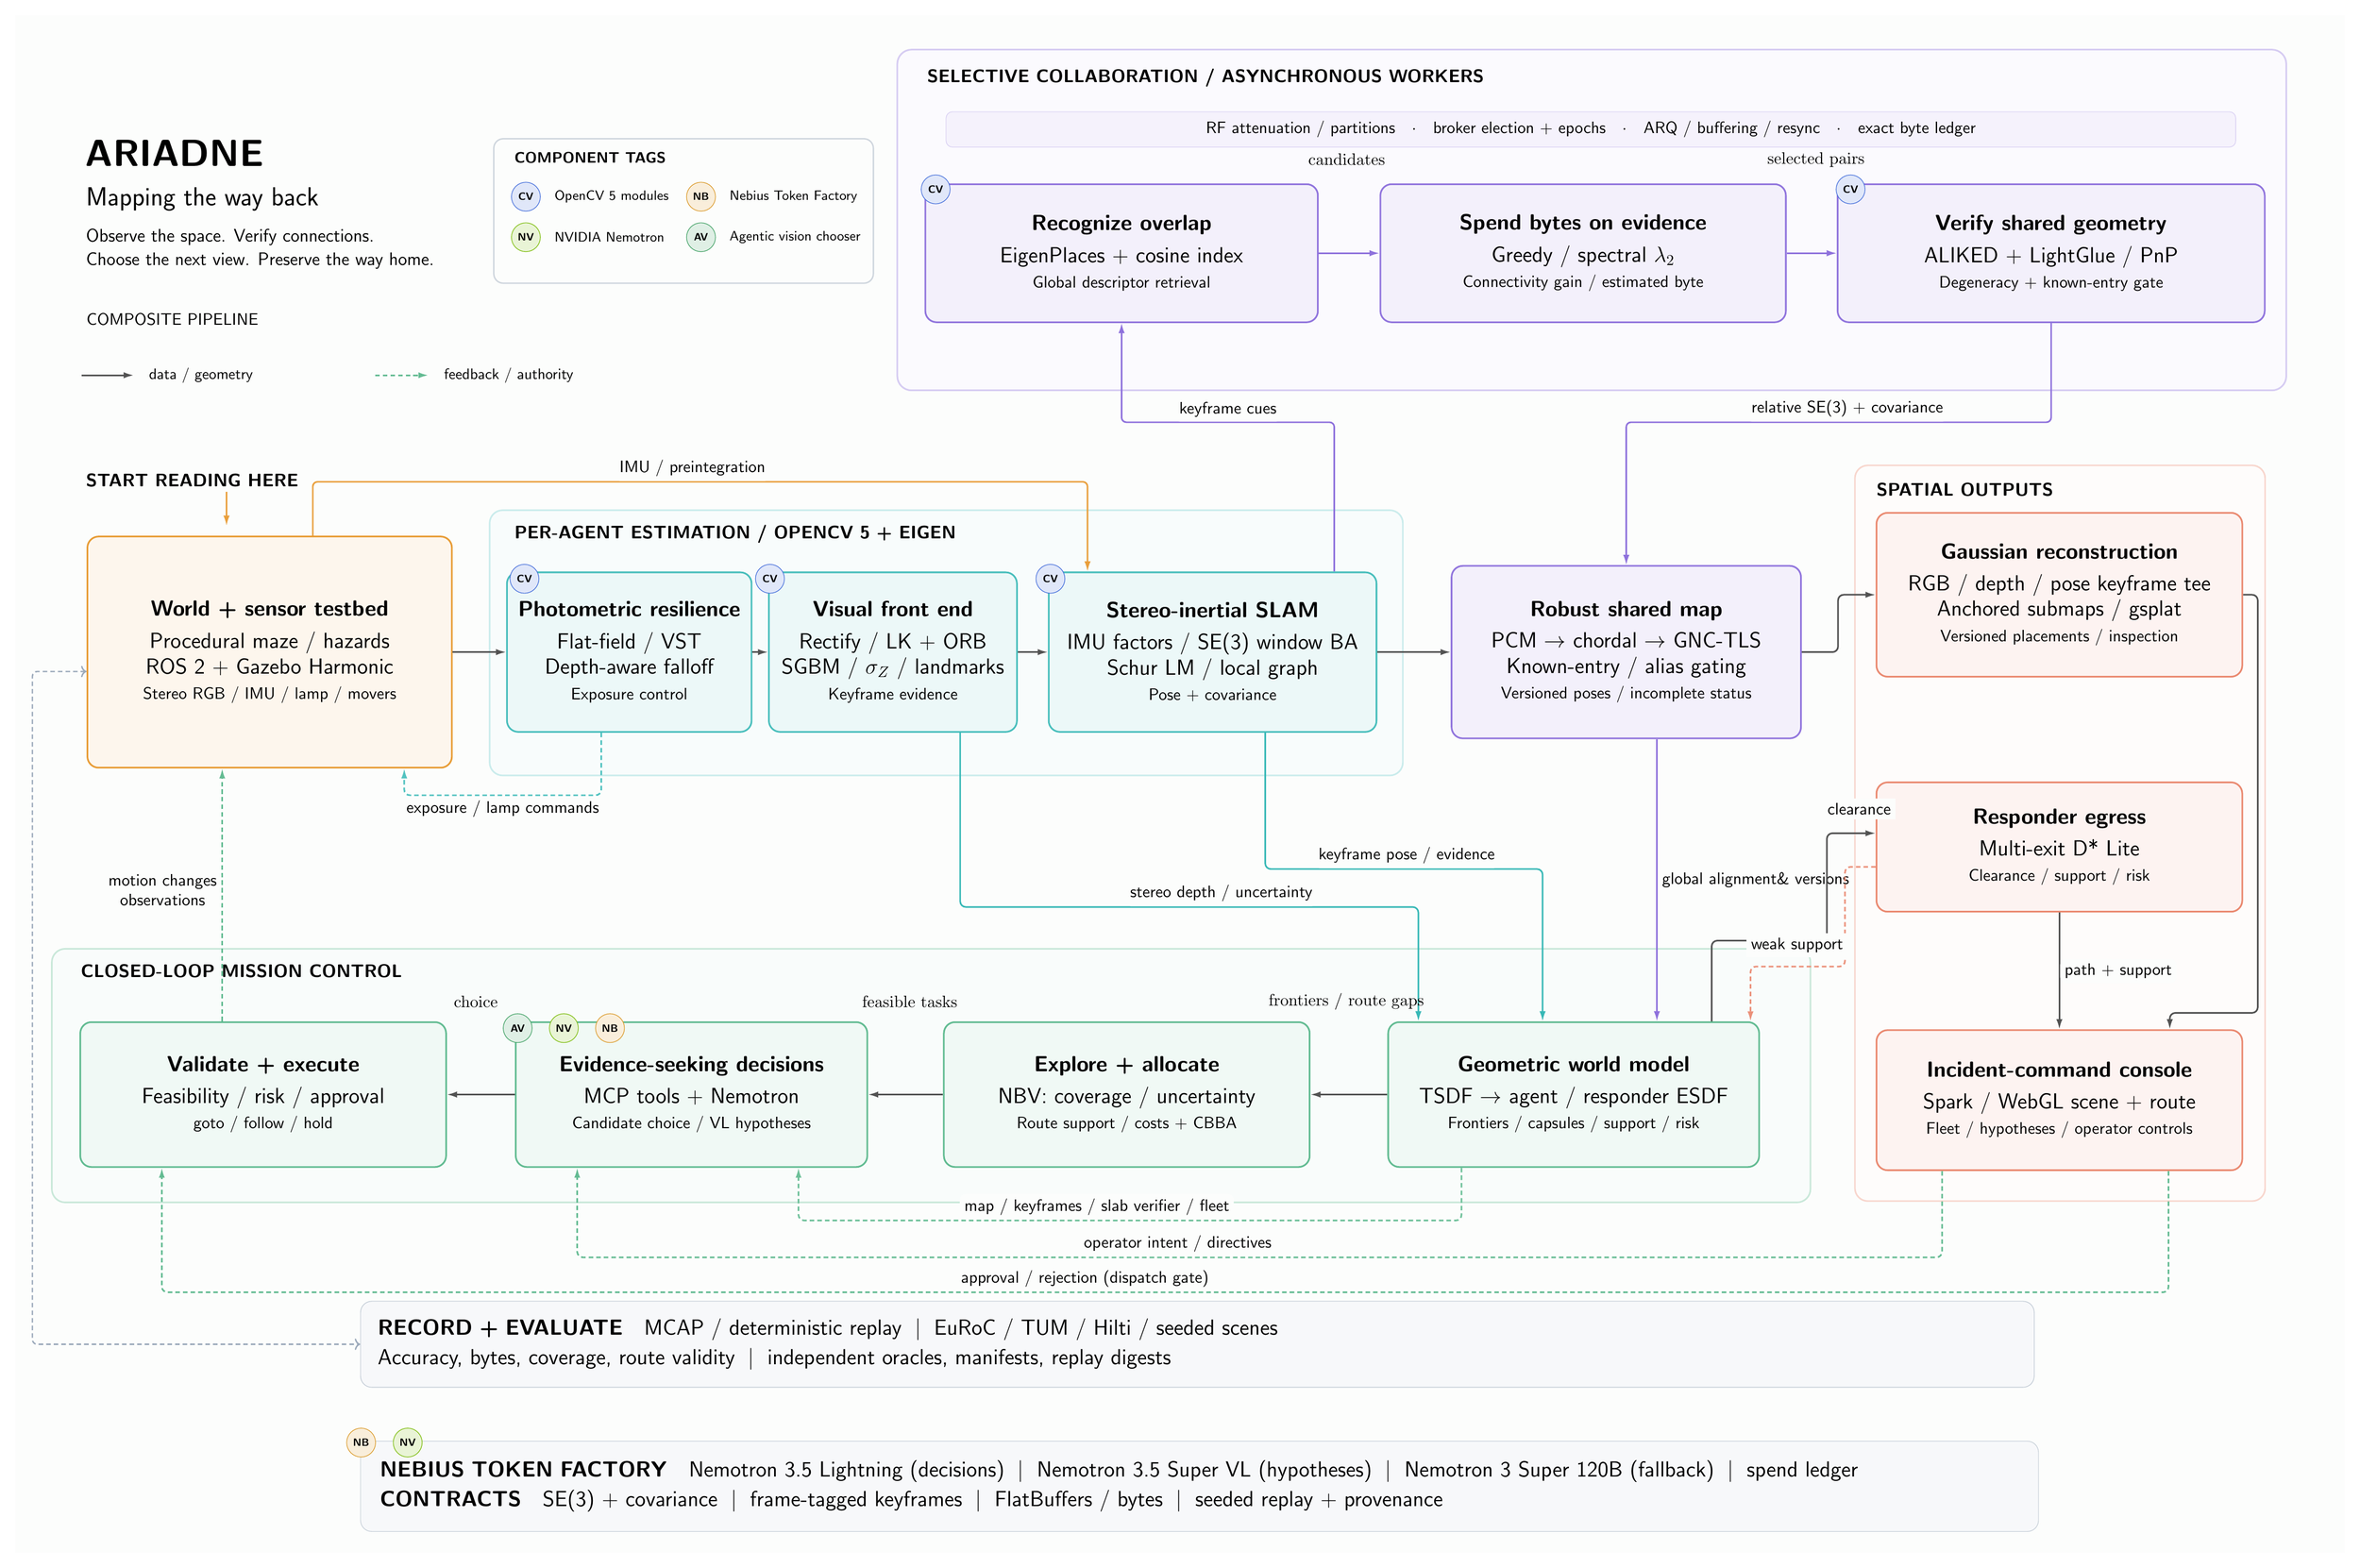
\begin{tikzpicture}[x=1cm,y=-1cm]
  \path[use as bounding box] (0,0) rectangle (54,35.65);
  \fill[paper] (0,0) rectangle (54,35.65);

\begin{scope}[shift={(\dxheader,\dyheader)}]
  \node[anchor=west,text=ink,font=\sffamily\fontsize{33}{36}\selectfont\bfseries] at (1.50,3.20) {ARIADNE};
  \node[anchor=west,text=ink,font=\sffamily\fontsize{18}{22}\selectfont] at (1.52,4.26) {Mapping the way back};
  \node[anchor=west,text=ink,font=\sffamily\fontsize{11.5}{14}\selectfont] at (1.52,5.15) {Observe the space. Verify connections.};
  \node[anchor=west,text=ink,font=\sffamily\fontsize{11.5}{14}\selectfont] at (1.52,5.69) {Choose the next view. Preserve the way home.};
  \node[anchor=west,text=ink,font=\sffamily\fontsize{10.6}{12}\selectfont] at (1.53,7.05) {COMPOSITE PIPELINE};
  \draw[flow] (1.54,8.35) -- (2.75,8.35);
  \node[anchor=west,text=ink,font=\sffamily\fontsize{10.2}{12}\selectfont] at (2.98,8.35) {data / geometry};
  \draw[control] (8.35,8.35) -- (9.58,8.35);
  \node[anchor=west,text=ink,font=\sffamily\fontsize{10.2}{12}\selectfont] at (9.82,8.35) {feedback / authority};
  \node[legendbox,anchor=north west,minimum width=8.8cm,minimum height=3.35cm] (legend) at (11.08,2.85) {};
  \node[anchor=west,text=ink,font=\sffamily\fontsize{10.4}{12}\selectfont\bfseries] at (11.45,3.31) {COMPONENT TAGS};
  \badgecv{11.84,4.21}
  \node[anchor=west,text=ink,font=\sffamily\fontsize{8.7}{10.8}\selectfont] at (12.38,4.21) {OpenCV 5 modules};
  \badgenv{11.84,5.15}
  \node[anchor=west,text=ink,font=\sffamily\fontsize{8.7}{10.8}\selectfont] at (12.38,5.15) {NVIDIA Nemotron};
  \badgenb{15.90,4.21}
  \node[anchor=west,text=ink,font=\sffamily\fontsize{8.7}{10.8}\selectfont] at (16.44,4.21) {Nebius Token Factory};
  \badgeagent{15.90,5.15}
  \node[anchor=west,text=ink,font=\sffamily\fontsize{8.7}{10.8}\selectfont] at (16.44,5.15) {Agentic vision chooser};
  \node[anchor=west,text=ink,font=\sffamily\fontsize{11.6}{13}\selectfont\bfseries] at (1.52,10.78) {START READING HERE};
  \draw[sensor] (4.9,11.05) -- (4.9,11.84);
\end{scope}

\begin{scope}[shift={(\dxcollab,\dycollab)}]
  \draw[rounded corners=3.3mm,draw=violet!28,fill=violet!3,line width=1.10pt] (20.45,0.80) rectangle (52.65,8.70);
  \node[laneheading,anchor=west,text=ink] at (21.02,1.46) {SELECTIVE COLLABORATION / ASYNCHRONOUS WORKERS};
  \node[rounded corners=1.5mm,draw=violet!28,fill=violet!7,anchor=center,text=ink,
        inner sep=1.4mm,minimum width=29.9cm,minimum height=.82cm,
        font=\sffamily\fontsize{11}{13.3}\selectfont] (transport) at (36.53,2.65)
        {RF attenuation / partitions\quad$\cdot$\quad broker election + epochs\quad$\cdot$\quad ARQ / buffering / resync\quad$\cdot$\quad exact byte ledger};
  \node[violetblock,minimum width=9.10cm,minimum height=3.2cm] (retrieve) at (25.65,5.52)
       {\textbf{Recognize overlap}\\[1.5mm]EigenPlaces + cosine index\\{\color{ink}\sffamily\fontsize{11.2}{13.6}\selectfont Global descriptor retrieval}};
  \badgecv{21.34,4.04}
  \node[violetblock,minimum width=9.40cm,minimum height=3.2cm] (select) at (36.35,5.52)
       {\textbf{Spend bytes on evidence}\\[1.5mm]Greedy / spectral $\lambda_2$\\{\color{ink}\sffamily\fontsize{11.2}{13.6}\selectfont Connectivity gain / estimated byte}};
  \node[violetblock,minimum width=9.90cm,minimum height=3.2cm] (verify) at (47.20,5.52)
       {\textbf{Verify shared geometry}\\[1.5mm]ALIKED + LightGlue / PnP\\{\color{ink}\sffamily\fontsize{11.2}{13.6}\selectfont Degeneracy + known-entry gate}};
  \badgecv{42.55,4.04}
  \draw[peer] (retrieve.east) -- (select.west);
  \node[tiny] at (30.87,3.35) {candidates};
  \draw[peer] (select.east) -- (verify.west);
  \node[tiny] at (41.75,3.35) {selected pairs};
\end{scope}

\begin{scope}[shift={(\dxmain,\dymain)}]
  \draw[rounded corners=3mm,draw=teal!22,fill=teal!3,line width=1.05pt] (11.0,11.48) rectangle (32.17,17.63);
  \node[laneheading,text=ink,anchor=west] at (11.45,12.03) {PER-AGENT ESTIMATION / OPENCV 5 + EIGEN};
  \node[orangeblock,minimum width=8.45cm,minimum height=5.36cm] (simulator) at (5.90,14.77)
     {\textbf{World + sensor testbed}\\[1.6mm]Procedural maze / hazards\\ROS 2 + Gazebo Harmonic\\{\color{ink}\sffamily\fontsize{11.2}{13.6}\selectfont Stereo RGB / IMU / lamp / movers}};
  \node[tealblock,minimum width=5.00cm,minimum height=3.70cm] (photo) at (14.2367,14.77)
     {\textbf{Photometric resilience}\\[1.5mm]Flat-field / VST\\Depth-aware falloff\\{\color{ink}\sffamily\fontsize{11.2}{13.6}\selectfont Exposure control}};
  \badgecv{11.8067,13.07}
  \node[tealblock,minimum width=5.75cm,minimum height=3.70cm] (frontend) at (20.3483,14.77)
     {\textbf{Visual front end}\\[1.5mm]Rectify / LK + ORB\\SGBM / $\sigma_Z$ / landmarks\\{\color{ink}\sffamily\fontsize{11.2}{13.6}\selectfont Keyframe evidence}};
  \badgecv{17.4983,13.07}
  \node[tealblock,minimum width=7.60cm,minimum height=3.70cm] (vio) at (27.76,14.77)
     {\textbf{Stereo-inertial SLAM}\\[1.5mm]IMU factors / SE(3) window BA\\Schur LM / local graph\\{\color{ink}\sffamily\fontsize{11.2}{13.6}\selectfont Pose + covariance}};
  \badgecv{24.00,13.07}
\end{scope}

\begin{scope}[shift={(\dxoutput,\dyoutput)}]
  \node[violetblock,minimum width=8.10cm,minimum height=4.00cm] (shared) at (37.35,14.77)
     {\textbf{Robust shared map}\\[1.4mm]PCM $\rightarrow$ chordal $\rightarrow$ GNC-TLS\\Known-entry / alias gating\\{\color{ink}\sffamily\fontsize{11.2}{13.6}\selectfont Versioned poses / incomplete status}};
  \draw[rounded corners=3mm,draw=coral!28,fill=coral!2,line width=1.03pt] (42.65,10.44) rectangle (52.16,27.50);
  \node[laneheading,anchor=west,text=ink] at (43.03,11.00) {SPATIAL OUTPUTS};
  \node[coralblock,minimum width=8.48cm,minimum height=3.80cm] (recon) at (47.39,13.44)
     {\textbf{Gaussian reconstruction}\\[1.4mm]RGB / depth / pose keyframe tee\\Anchored submaps / gsplat\\{\color{ink}\sffamily\fontsize{11.2}{13.6}\selectfont Versioned placements / inspection}};
  \node[coralblock,minimum width=8.48cm,minimum height=3.00cm] (route) at (47.39,19.29)
     {\textbf{Responder egress}\\[1.4mm]Multi-exit D* Lite\\{\color{ink}\sffamily\fontsize{11.2}{13.6}\selectfont Clearance / support / risk}};
  \node[coralblock,minimum width=8.48cm,minimum height=3.25cm] (console) at (47.39,25.16)
     {\textbf{Incident-command console}\\[1.4mm]Spark / WebGL scene + route\\{\color{ink}\sffamily\fontsize{11.2}{13.6}\selectfont Fleet / hypotheses / operator controls}};
\end{scope}

\begin{scope}[shift={(\dxmission,\dymission)}]
  \draw[rounded corners=3.1mm,draw=greenx!26,fill=greenx!3,line width=1.05pt] (.85,21.65) rectangle (41.62,27.53);
  \node[laneheading,anchor=west,text=ink] at (1.40,22.16) {CLOSED-LOOP MISSION CONTROL};
  \node[greenblock,minimum width=8.48cm,minimum height=3.36cm] (dispatch) at (5.75,25.03)
     {\textbf{Validate + execute}\\[1.4mm]Feasibility / risk / approval\\{\color{ink}\sffamily\fontsize{11.2}{13.6}\selectfont goto / follow / hold}};
  \node[greenblock,minimum width=8.15cm,minimum height=3.36cm] (chooser) at (15.68,25.03)
     {\textbf{Evidence-seeking decisions}\\[1.4mm]MCP tools + Nemotron\\{\color{ink}\sffamily\fontsize{11.2}{13.6}\selectfont Candidate choice / VL hypotheses}};
  \badgeagent{11.65,23.49}\badgenv{12.72,23.49}\badgenb{13.79,23.49}
  \node[greenblock,minimum width=8.48cm,minimum height=3.36cm] (nbv) at (25.77,25.03)
     {\textbf{Explore + allocate}\\[1.4mm]NBV: coverage / uncertainty\\{\color{ink}\sffamily\fontsize{11.2}{13.6}\selectfont Route support / costs + CBBA}};
  \node[greenblock,minimum width=8.60cm,minimum height=3.36cm] (volume) at (36.13,25.03)
     {\textbf{Geometric world model}\\[1.4mm]TSDF $\rightarrow$ agent / responder ESDF\\{\color{ink}\sffamily\fontsize{11.2}{13.6}\selectfont Frontiers / capsules / support / risk}};
\end{scope}

\draw[flow] (simulator.east) -- (photo.west);
\draw[flow] (photo.east) -- (frontend.west);
\draw[flow] (frontend.east) -- (vio.west);
\draw[flow] (vio.east) -- (shared.west);

\coordinate (imuout) at ($(simulator.north)+(1.00cm,0cm)$);
\coordinate (imuin)  at ($(vio.north)+(-2.90cm,0cm)$);
\coordinate (imuRail) at ($(imuout)+(0,1.25cm)$);
\draw[sensor] (imuout) -- (imuout |- imuRail)
  -- node[lab,above,pos=.49]{IMU / preintegration} (imuin |- imuRail) -- (imuin);

\coordinate (cuesout) at ($(vio.north)+(2.82cm,0cm)$);
\coordinate (collabRail) at ($(retrieve.south)+(0,-2.30cm)$);
\draw[peer] (cuesout) -- (cuesout |- collabRail)
  -- node[lab,above,pos=.5]{keyframe cues} (retrieve.south |- collabRail) -- (retrieve.south);
\draw[peer] (verify.south) -- (verify.south |- collabRail)
  -- node[lab,above,pos=.48]{relative SE(3) + covariance} (shared.north |- collabRail) -- (shared.north);

\coordinate (photoright) at ($(photo.south)+(-.65cm,0cm)$);
\coordinate (actuator) at ($(simulator.south)+(3.12cm,0cm)$);
\coordinate (photoRail) at ($(photoright)+(0,-1.45cm)$);
\draw[control,draw=teal!72] (photoright) -- (photoright |- photoRail)
  -- node[lab,below,pos=.5]{exposure / lamp commands} (actuator |- photoRail) -- (actuator);

\coordinate (depthout) at ($(frontend.south)+(1.56cm,0cm)$);
\coordinate (depthin) at ($(volume.north)+(-3.60cm,0cm)$);
\coordinate (depthRail) at ($(volume.north)+(0,2.65cm)$);
\draw[data] (depthout) -- (depthout |- depthRail)
  -- node[lab,above,pos=.57]{stereo depth / uncertainty} (depthin |- depthRail) -- (depthin);
\coordinate (poseout) at ($(vio.south)+(1.22cm,0cm)$);
\coordinate (posein) at ($(volume.north)+(-.72cm,0cm)$);
\coordinate (poseRail) at ($(volume.north)+(0,3.53cm)$);
\draw[data] (poseout) -- (poseout |- poseRail)
  -- node[lab,above,pos=.51]{keyframe pose / evidence} (posein |- poseRail) -- (posein);
\coordinate (versionin) at ($(volume.north)+(1.93cm,0cm)$);
\coordinate (versionout) at (versionin |- shared.south);
\draw[peer] (versionout) -- node[lab,right]{global alignment\& versions} (versionin);

\coordinate (anchorRail) at ($(shared.east)+(.84cm,0cm)$);
\draw[flow] (shared.east) -- (anchorRail)
  -- (anchorRail |- recon.west) -- (recon.west);

\draw[flow] (volume.west) -- (nbv.east);
\node[tiny] at (30.86,22.88) {frontiers / route gaps};
\draw[flow] (nbv.west) -- (chooser.east);
\node[tiny] at (20.74,22.88) {feasible tasks};
\draw[flow] (chooser.west) -- (dispatch.east);
\node[tiny] at (10.68,22.88) {choice};

\coordinate (movein) at ($(simulator.south)+(-1.1cm,0cm)$);
\coordinate (moveout) at (movein |- dispatch.north);
\draw[control] (moveout) -- node[lab,left,pos=.52]{motion changes\\observations} (movein);

\coordinate (clearout) at ($(volume.north)+(3.2cm,0cm)$);
\coordinate (clearin) at ($(route.west)+(0cm,.32cm)$);
\coordinate (clearanceRail) at ($(volume.north)+(0,1.87cm)$);
\coordinate (clearanceColumn) at (42.00,0);
\draw[flow] (clearout) -- (clearout |- clearanceRail)
  -- (clearanceColumn |- clearanceRail) -- (clearanceColumn |- clearin) -- (clearin);
\node[lab,above] at (42.75,18.65) {clearance};
\coordinate (uncout) at ($(route.west)+(0cm,-.46cm)$);
\coordinate (uncin) at ($(volume.north)+(4.1cm,0cm)$);
\coordinate (supportColumn) at (42.42,0);
\coordinate (supportRail) at ($(volume.north)+(0,1.27cm)$);
\draw[control,draw=coral!75] (uncout) -- (supportColumn |- uncout)
  -- (supportColumn |- supportRail) -- (uncin |- supportRail) -- (uncin);
\node[lab,above] at (41.31,21.85) {weak support};

\coordinate (reconConsoleColumn) at ($(recon.east)+(.34cm,0cm)$);
\coordinate (consoleIn) at ($(console.north)+(2.56cm,0cm)$);
\coordinate (consoleRail) at ($(consoleIn)+(0,.38cm)$);
\draw[flow] (recon.east) -- (reconConsoleColumn)
  -- (reconConsoleColumn |- consoleRail) -- (consoleRail) -- (consoleIn);
\draw[flow] (route.south) -- node[lab,right]{path + support} (console.north);

\coordinate (contextout) at ($(volume.south)+(-2.6cm,0cm)$);
\coordinate (contextin) at ($(chooser.south)+(2.48cm,0cm)$);
\coordinate (contextRail) at ($(volume.south)+(0,-1.22cm)$);
\draw[control,draw=greenx!70] (contextout) -- (contextout |- contextRail)
  -- node[lab,above,pos=.55]{map / keyframes / slab verifier / fleet} (contextin |- contextRail) -- (contextin);

\coordinate (intentout) at ($(console.south)+(-2.72cm,0cm)$);
\coordinate (approvalout) at ($(console.south)+(2.53cm,0cm)$);
\coordinate (intentin) at ($(chooser.south)+(-2.65cm,0cm)$);
\coordinate (approvalin) at ($(dispatch.south)+(-2.35cm,0cm)$);
\coordinate (intentRail) at ($(console.south)+(0,-2.00cm)$);
\coordinate (approvalRail) at ($(console.south)+(0,-2.81cm)$);
\draw[control] (intentout) -- (intentout |- intentRail)
  -- node[lab,above,pos=.56]{operator intent / directives} (intentin |- intentRail) -- (intentin);
\draw[control] (approvalout) -- (approvalout |- approvalRail)
  -- node[lab,above,pos=.54]{approval / rejection (dispatch gate)} (approvalin |- approvalRail) -- (approvalin);

\begin{scope}[shift={(\dxevidence,\dyevidence)}]
 \node[rounded corners=\roundr,draw=infra!45,fill=infra!5,anchor=west,text=ink,
    inner sep=4mm,text width=38.0cm,font=\sffamily\fontsize{13.9}{17.9}\selectfont] (evidence) at (8.0,30.82)
    {\textbf{RECORD + EVALUATE}\quad MCAP / deterministic replay $\;|\;$ EuRoC / TUM / Hilti / seeded scenes\\[.6mm]
     Accuracy, bytes, coverage, route validity $\;|\;$ independent oracles, manifests, replay digests};
\end{scope}
\coordinate (recordPort) at ($(simulator.west)+(0cm,-.45cm)$);
\coordinate (recordColumn) at (.40,0);
\draw[rail,<->] (recordPort) -- (recordColumn |- recordPort)
  -- (recordColumn |- evidence.west) -- (evidence.west);
\begin{scope}[shift={(\dxinfer,\dyinfer)}]
 \node[rounded corners=\roundr,draw=infra!40,fill=infra!5,anchor=north west,text=ink,
    inner sep=4.5mm,text width=38.0cm,font=\sffamily\fontsize{13.9}{17.9}\selectfont] (infer) at (8.0,33.06)
    {\textbf{NEBIUS TOKEN FACTORY}\quad Nemotron 3.5 Lightning (decisions) $\;|\;$ Nemotron 3.5 Super VL (hypotheses) $\;|\;$ Nemotron 3 Super 120B (fallback) $\;|\;$ spend ledger\\[.6mm]
     \textbf{CONTRACTS}\quad SE(3) + covariance $\;|\;$ frame-tagged keyframes $\;|\;$ FlatBuffers / bytes $\;|\;$ seeded replay + provenance};
  \badgenb{8.02,33.10}\badgenv{9.10,33.10}
\end{scope}

\end{tikzpicture}
\end{document}
